\chapter{Defenses}
\label{chp:defenses}
In the previous chapter, we successfully performed several targeted item-to-item attacks that allow an attacker to promote their items by adding almost imperceptible perturbations to product images. These findings raise a fundamental question:
\begin{center}
	\textit{How can we defend our recommendation system against adversarial inputs?}
\end{center} 
There is now a sizable body of work proposing various defense mechanisms against adversarial examples. Even though researchers have published many different defense techniques, the research area is still relatively young \parencite{szegedy2013intriguing}, and new studies frequently circumvent a lot of published defenses. A prominent example of such a study was published by \cite{athalye2018obfuscated}. They evaluated nine non-certified white-box-secure defenses published at the ICLR 2018 conference and identified obfuscated gradients, a phenomenon that leads to a false sense of security in defenses against adversarial examples. Out of the nine evaluated defenses, they circumvented six completely, and one partially. Two defenses were considered useful, and are both based on the idea of \ac{AT}. Hence we also based our experiments on defenses belonging to this class. We evaluate using these defense techniques to train our \ac{CNN} feature extractor in the following sections and show the impact these defenses have on our proposed attacks against our \ac{k-NN} recommendation system. 

\section{Adversarial Training}
Starting with vanilla adversarial training, we study the approach of \cite{madry2017towards}. During the adversarial training procedure, we instantiate the attack used of our \ac{CNN} feature extractor with \ac{PGD} using eight iterations and restricting $l_\infty$ perturbations to $\epsilon=0.03$. In contrast to our item-to-item attacks performed in Chapter~\ref{chp:attacks}, our adversary objective during adversarial training, is to increase the likelihood of misclassification for the category, and texture attributes. We perform the adversarial training for 24 epochs, as we did for our regular classifier. 

Looking at the evaluation metrics for our classifier in Table~\ref{tab:adv-classifier-results}, we can see that, as expected, our performed attacks reduced our regular classifier performance drastically, while our adversarially trained classifier was able to learn a more robust decision boundary.  This increase in robustness is traded in for a decrease in accuracy on clean images. In our case, the accuracy for the adversarially trained model in predicting the correct garment category dropped by 12.19\% on clean images, while we gained 48.69\% for the same task on adversarial images. Similar results can be seen for the multi-class task of texture classification. This trade-off is well-known and has been attributed to the fundamental conflict between the goal of adversarial robustness and that of standard generalization \parencite{tsipras2018robustness}.
\begin{table}[H]
	\centering
	\subfloat[][Category classification results.]{
		\label{tab:adv-category-results}
		\begin{tabular}{ lccc } 
			\toprule		
			Category        	 & Adversarial & Regular & $\Delta$\\
			\midrule
			Clean Accuracy	     & 56.06 & 68.25 & $-$ 12.19 \\
			Adversarial Accuracy & 48.71 & 0.02  & $+$ 48.69  \\
			\bottomrule
		\end{tabular}
	}
	\hfill
	\subfloat[][Texture classification results.]{
		\label{tab:adv-texture-results}
		\begin{tabular}{ lccc } 
			\toprule		
			Texture          			& Adversarial & Regular & $\Delta$ \\
			\midrule
			Clean Top-1 Precision       & 39.58 & 43.68 & $-$ 4.10 \\
			Adversarial Top-1 Precision & 38.60 & 19.51 & $+$ 19.09 \\
			\bottomrule
		\end{tabular}
	}
	\caption{Comparison of our evaluation results on a clean and adversarial test set for a adversarially trained and regular classifier. The adversarial test set was generated using the \ac{PGD} attack method with eight iterations and $\epsilon=0.03$.}
	\label{tab:adv-classifier-results}
\end{table}
Since we are interested in evaluating if this kind of training procedure can help us mitigate the attacks on our \ac{k-NN} recommendation system, we evaluate the success rates of our previously proposed attacks against our adversarially trained feature extractor. To get a first impression, we try to reproduce our targeted attacks on the same attack tuple that we used to demonstrate our attacks in the previous chapter. With relatively low epsilon values up to 0.05, which were enough to reach 99.70\% attack success rate for our undefended model, as seen in Table~\ref{tab:attack-results}, we fail to achieve a significant rank with our adversarial examples. Even with unrealistically high epsilon values like 0.3, we still fail to rank under the ten nearest neighbors, as seen in Figure~\ref{fig:adv-reco}. Interestingly, for the adversarially trained model, the adversarial images with high epsilon values start to show relevant features of the target image. For example, in Figure~\ref{fig:epsilon-adv}, the stripes of the striped sweater start to appear in the adversarial image. This phenomenon does not occur for our regular model and might indicate that our adversarially trained model learned more relevant features, which help it defend against unrealistic manipulations of the input. 
\begin{figure}[H]
	\centering
	\begin{tikzpicture}

\node [rectangle, inner sep=0.5pt, color1, draw, thick] (query1) {\includegraphics[width=2.25cm] {../../data/DeepFashion/img_resized/Striped_Textured_Sweater/img_00000024.jpg}};
\node [above=of query1, yshift=-1cm, color1, font=\small] {\textbf{Query} image};


\node [right=of query1, rectangle, inner sep=0.5pt, color2, draw, thick] (orig1) {\includegraphics[width=2cm] {../../data/DeepFashion/img_resized/Flat_Collar_Woven_Blouse/img_00000034.jpg}};
\node [above=of orig1, yshift=-1cm, color2, font=\small] {$dist = 0.0306$};

\node [right=0.5cm of orig1, rectangle, inner sep=0.5pt, color2, draw, thick] (orig2) {\includegraphics[width=2cm] {../../data/DeepFashion/img_resized/Nautical_Stripe_Jersey_Tee/img_00000018.jpg}};
\node [above=of orig2, yshift=-1cm, color2, font=\small] {$dist = 0.0350$};

\node [right=0.5cm of orig2, rectangle, inner sep=0.5pt, color2, draw, thick] (orig3) {\includegraphics[width=2cm] {../../data/DeepFashion/img_resized/Classic_Striped_Top/img_00000032.jpg}};
\node [above=of orig3, yshift=-1cm, color2, font=\small] {$dist = 0.0434$};

\node [right=0.5cm of orig3, rectangle, inner sep=0.5pt, color2, draw, thick] (orig4) {\includegraphics[width=2cm] {../../data/DeepFashion/img_resized/Boxy_Stripe_Sweater/img_00000029.jpg}};
\node [above=of orig4, yshift=-1cm, color2, font=\small] {$dist = 0.0446$};


\end{tikzpicture}
	\caption{A recommendation result of our adversarially trained model after a targeted attack. The  adversarial example generated using the \ac{CW} method for $\epsilon=0.3$, which we injected into the product catalog ranks on place 39 and is therefore not visible in the nearest neighbors displayed above.}
	\label{fig:adv-reco}
\end{figure}
\begin{figure}[H]
	\centering
	\subfloat[][$\epsilon=0.01$]{
		\includegraphics[height=0.18\textwidth]{images/adv/adversarial-24-epochs/cw/0.01/attack}
	}
	\subfloat[][$\epsilon=0.05$]{
		\includegraphics[height=0.18\textwidth]{images/adv/adversarial-24-epochs/cw/0.05/attack}
	}
	\subfloat[][$\epsilon=0.1$]{
		\includegraphics[height=0.18\textwidth]{images/adv/adversarial-24-epochs/cw/0.1/attack}
	}
	\subfloat[][$\epsilon=0.2$]{
		\includegraphics[height=0.18\textwidth]{images/adv/adversarial-24-epochs/cw/0.2/attack}
	}
	\subfloat[][$\epsilon=0.3$]{
		\includegraphics[height=0.18\textwidth]{images/adv/adversarial-24-epochs/cw/0.3/attack}
	}
	\caption{Adversarial examples generated using \acs{CW}-1000 for our adversarially trained recommendation system with increasing $\epsilon$ values ranging from 0.01 to 0.3. The target item for the attack is the same striped sweater as in Chapter~\ref{chp:attacks}.}
	\label{fig:epsilon-adv}
\end{figure}
The first impression of the robustness characteristics regarding our proposed attacks is confirmed, when we look at the empirical evaluation results over a broader set of article tuples in Table~\ref{tab:adv-training-results} and Figure~\ref{fig:top3-adv-success}. Using adversarial training, we were able to reduce the attack success rate for a perturbation budget of $\epsilon=0.05$ from 99.70\% to a mere 0.30\%. When we look at higher and more noticeable perturbation budgets $\epsilon\ge0.1$, the success rates start to increase slowly. The \ac{CW} method once again strongly outperforms all other tested methods, demonstrating its superior effectiveness at navigating the loss surface of adversarial examples. We conclude that the achieved reduction in success rates for realistic $\epsilon$ values $\le$ 0.05, makes successful attacks impractical, as users would likely notice the manipulation for higher $\epsilon$ values and the degradation in image quality reaches unacceptable levels.

Inspecting the impact of \ac{AT} on cosine distances, before and after \ac{CW} attacks, in Figure~\ref{fig:adv-quantile}, we observe a reassuring pattern. The majority of the points are very close to the plot's identity or have only been reduced by a constant amount, indicating that \ac{AT} can indeed be considered an efficient defense mechanism for our use-case.
\begin{table}[H]
	\centering
	\begin{tabular}{ lccccc } 
		\toprule		
		& \multicolumn{5}{c}{Maximal Perturbation} \\
		\cmidrule{2-6}
		Attack & $\epsilon = 0.01$ & $\epsilon = 0.05$ & $\epsilon = 0.1$  & $\epsilon = 0.2$ & $\epsilon = 0.3$  \\
		\midrule
		FGSM & 0.01 & 0.03 & 0.02 & 0.02 & 0.00 \\
		PGD-8 & 0.01 & 0.07 & 0.42 & 3.18 & 6.91 \\
		PGD-16 & 0.01 & 0.07 & 0.48 & 4.33 & 12.04 \\
		PGD-32 & 0.01 & 0.07 & 0.48 & 5.12 & 15.43 \\
		PGD-64 & 0.01 & 0.07 & 0.50 & 5.45 & 16.97 \\
		PGD-128 & 0.01 & 0.07 & 0.53 & 5.61 & 17.68 \\
		CW-1000 & 0.00 & 0.30 & 1.80 & 23.10 & 48.00 \\
		\bottomrule
	\end{tabular}
	\caption{Attack success rates for $rank_{min}=3$, targeting an adversarially trained model, calculated over 10,000 random article tuples (1,000 in the case of \acs{CW}) for all evaluated attacks and various $\epsilon$ values.}
	\label{tab:adv-training-results}
\end{table}
\begin{figure}[H]
	\centering
	\input{images/top3-adv-success}
	\caption{Attack success rates for $rank_{min}=3$, targeting an adversarially trained model, calculated over 10,000 random article tuples (1,000 in the case of \acs{CW}) for all evaluated attacks and various $\epsilon$ values.}
	\label{fig:top3-adv-success}
\end{figure}
\begin{figure}[H]
	\centering
	% This file was created by tikzplotlib v0.9.3.
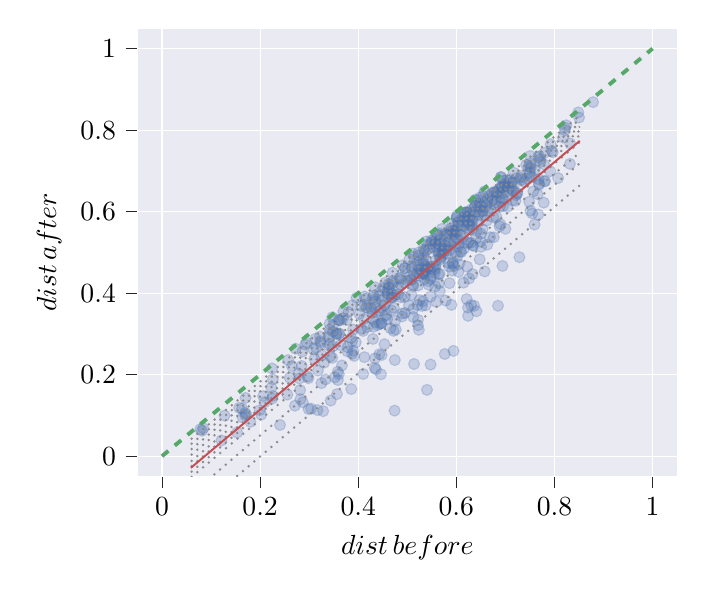
\begin{tikzpicture}

\definecolor{color0}{rgb}{0.917647058823529,0.917647058823529,0.949019607843137}
\definecolor{color1}{rgb}{0.298039215686275,0.447058823529412,0.690196078431373}
\definecolor{color2}{rgb}{0.768627450980392,0.305882352941176,0.32156862745098}
\definecolor{color3}{rgb}{0.333333333333333,0.658823529411765,0.407843137254902}

\begin{axis}[
axis background/.style={fill=color0},
axis line style={white},
tick align=outside,
tick pos=left,
x grid style={white},
xlabel={$dist\,before$},
xmajorgrids,
xmin=-0.05, xmax=1.05,
xtick style={color=white!15!black},
y grid style={white},
ylabel={$dist\,after$},
ymajorgrids,
ymin=-0.05, ymax=1.05,
ytick style={color=white!15!black}
]
\addplot [only marks, mark=*, draw=color1, fill=color1, opacity=0.25, colormap/blackwhite, clip marker paths=true]
table{%
x                      y
0.733669391358075 0.677763807674963
0.600792870061178 0.53253845164843
0.566333974654135 0.545942899640457
0.559145759298773 0.378772719963487
0.537456225696392 0.370007807777585
0.421510116149886 0.362335570856807
0.699766245539921 0.663772957169746
0.591686463098158 0.570686686657271
0.699033425099298 0.663583947323067
0.656266661868739 0.624071274106261
0.328548528400302 0.110345127815428
0.596068368797792 0.548742512598244
0.297135447186903 0.195535219497771
0.622286807344624 0.464744739365445
0.691687147564503 0.625669682595825
0.641586001351707 0.552682354073893
0.506104960641207 0.442338887633811
0.157228433085191 0.118653042659483
0.169678723757314 0.0996566575636835
0.564454974530201 0.424171663689042
0.523031419408563 0.499806876861342
0.322129674402128 0.293512103152662
0.413420437617521 0.371948488793355
0.452574248813613 0.369118205620786
0.603356201466969 0.513936157436808
0.402484363042664 0.348939265667696
0.625739997151201 0.570206821677885
0.343164646210649 0.24498253182073
0.657746020943439 0.453330340163536
0.342319043539444 0.310941648420485
0.594129662782021 0.258313817922206
0.455271587000315 0.425688513488409
0.679312797994057 0.647339591195556
0.415278727848808 0.386454118348233
0.757051906780796 0.649721483193764
0.513226211014756 0.488606235699876
0.257051972465874 0.235838719748025
0.521229158533449 0.449097939116283
0.548096551806037 0.441540079823615
0.64874001892406 0.635163786726693
0.663811233594638 0.620864664647842
0.481156486928423 0.397411109816886
0.623238328757117 0.522279597834319
0.535322258596357 0.464329565314812
0.695689281458672 0.645029175336043
0.594314516872237 0.553628176760564
0.529859995842906 0.368335219097534
0.523622844810017 0.31007257750825
0.562468472535884 0.54155190057854
0.489605788176018 0.34985720057163
0.447776304562541 0.248126409289069
0.732179136044367 0.687871922037348
0.27810484439288 0.202827804994766
0.426485382827624 0.362014286406323
0.495123324483822 0.461828672429323
0.677651313803879 0.648892938809713
0.298347024327579 0.191344376442603
0.470577652788228 0.423549469870456
0.433488527600813 0.216642853824538
0.358453392716211 0.186781880412263
0.750382085532852 0.717963501820167
0.360604080245056 0.201305133546486
0.557416516798029 0.460539208037334
0.621554775177371 0.596444802104406
0.308882282177038 0.261891146140702
0.341586842508674 0.324673132206278
0.778676877375931 0.716017852419911
0.396533742327839 0.388556346840363
0.431582423710743 0.393742323982178
0.559843304462181 0.511611878008798
0.524600527933603 0.442734274526248
0.711922499292714 0.655238783114135
0.495348467021198 0.351348531309409
0.32251833982407 0.282316592511871
0.494729227014707 0.460529590726181
0.281479094812251 0.162284547207421
0.507022422100435 0.432386507832137
0.378151851507503 0.257021720191977
0.640187815671559 0.598887722513514
0.690929396673754 0.685276210223111
0.648239694260054 0.598968033631504
0.650630254881328 0.590467716662697
0.446455516755634 0.200952234489714
0.627016614042637 0.567140509527219
0.490301238750084 0.468132888947413
0.778198662667451 0.622025697200692
0.689458560809748 0.569302321199774
0.601389667577866 0.589353504582251
0.294456695574698 0.278911070874986
0.121268917206039 0.0384896453334959
0.476620413591845 0.310521016708509
0.621117457465856 0.385575408669783
0.169428343160155 0.106158297277241
0.567378149128596 0.48207941401372
0.385787771998174 0.164702885334566
0.636417309841116 0.368879951658801
0.487099654116088 0.389713065839695
0.692609063828733 0.65890386081386
0.791465579620137 0.699144509016015
0.691473389229572 0.662397668825484
0.522697276891388 0.464126787707988
0.588596727869425 0.553023058564422
0.513091346616812 0.445711140497877
0.680828563655856 0.622424753468751
0.633136875940941 0.577562297958032
0.504339563378366 0.483397388904886
0.529612462361058 0.448064243423545
0.430930810940021 0.336081090240911
0.380162432336596 0.353581187795439
0.688556767846399 0.612109311943771
0.647550657264595 0.482802308694241
0.69525257656425 0.61361694850584
0.722040650190699 0.681972555560724
0.65350254789465 0.602631333977966
0.616134804193989 0.563914193659242
0.605477945457727 0.470856004209722
0.616197154032886 0.596997815422913
0.468434158023644 0.398480277551246
0.434442152376944 0.328779274189308
0.366832460509277 0.222591319777371
0.508684721110615 0.395653779278673
0.531838498155986 0.380019681627186
0.358269161758412 0.207009634972667
0.352154134221025 0.193234611386966
0.653474522128707 0.556791086578617
0.593175336338297 0.47524990124374
0.314148076364412 0.265699048340509
0.389574211746678 0.310438020648453
0.525953657438257 0.479224330889613
0.413019387423465 0.391643789922366
0.376933818690317 0.334099525692893
0.643740768243927 0.59281590671508
0.751007036023505 0.602023616049232
0.209343049994959 0.132347697972052
0.512103481875332 0.417449194333043
0.759827807195084 0.702216350229546
0.55916962251337 0.481027224092767
0.630872057668515 0.580701798630174
0.127535283723867 0.0995633523594606
0.650386875737865 0.513703689551442
0.51712425172184 0.470338936406414
0.556096846321517 0.449989589476637
0.623966762106398 0.344229193368213
0.585723739466451 0.465072387857756
0.562413337472743 0.500991044325961
0.688977492995426 0.642278589257441
0.693303682890779 0.633464764334042
0.368916959788073 0.338574565688319
0.52524367330109 0.383039810509068
0.600239974641114 0.582857183693673
0.618764353143386 0.586136688348002
0.171841151615669 0.102759823413356
0.652074269785705 0.613093070233712
0.541196432485508 0.463928543176962
0.540254788581927 0.162643935070267
0.48575643573394 0.438093568139918
0.522009549448938 0.418636271790292
0.33044690700322 0.22933883507808
0.533385690509705 0.446527861143311
0.684962180834748 0.369027232691819
0.341824295540519 0.274904845578836
0.748772786522185 0.692330267883841
0.388201469894698 0.370192201350399
0.705413331475689 0.661593971524388
0.807509633170375 0.682367469528834
0.593717494409354 0.549613298913008
0.0840901128773099 0.0687281531875508
0.317810475303331 0.210342119246746
0.792335744946186 0.76539785830644
0.343847108239607 0.136329527079049
0.312601535939725 0.287922104314878
0.663327571106794 0.601756947406126
0.390197468252239 0.25848993470947
0.587615260303793 0.544435542784756
0.578089856109601 0.381650110930659
0.360632736916652 0.299506563247787
0.557090576899401 0.416843886270099
0.586150395771891 0.424529825589659
0.525052616268837 0.457585780852718
0.681843605280663 0.648358307584481
0.406532524545915 0.312603661299534
0.454119609789875 0.343250659517249
0.462268045200672 0.422957387248291
0.627911297092938 0.598853396768916
0.663183821302186 0.518920979515274
0.566153233210296 0.521206277661036
0.638109798093142 0.613377386080446
0.723277987398226 0.646049272075929
0.688167577790908 0.563946244918573
0.70272051518956 0.649592014636125
0.470080826160041 0.450229133759166
0.616481296850928 0.58376614070178
0.444387995389751 0.324438237359925
0.509502930764524 0.460096795824759
0.359629420093282 0.334357908268824
0.486811048538914 0.432742960496999
0.622493261945558 0.561585930181235
0.648905755289096 0.526316050591484
0.500347737488413 0.430840304434675
0.696181346842337 0.630389841545473
0.521715816812562 0.321287364596801
0.57136638094257 0.499859224708175
0.287081360463044 0.132272715024965
0.640428512872614 0.534497979967183
0.650176356502943 0.545966075702748
0.412750966575225 0.242861601208676
0.325193825296416 0.247360851834932
0.769117876035416 0.735631725236332
0.832085019205161 0.767009573406775
0.348864711184576 0.321103028157871
0.565206005859736 0.520144509311857
0.821468756709336 0.799660291082354
0.739311758130885 0.672892367469783
0.395114584569757 0.279194394009448
0.630206628132733 0.370442146355466
0.779856861227799 0.744410445066498
0.355393816455584 0.300801809314021
0.391616248017617 0.246014483922655
0.44191577629182 0.354524095455124
0.468409921352951 0.3905800315204
0.170329699244582 0.142892838676891
0.264754694934734 0.22098750939387
0.0816554742042784 0.0624190654170366
0.467624302834744 0.39017202203919
0.831526032585375 0.717159877986583
0.75156908797838 0.711042686019532
0.771549834652583 0.721800528837051
0.619969696615958 0.598218069925624
0.584253445824044 0.474140989647815
0.566236447613462 0.405029996982901
0.323861212685636 0.278268336926029
0.662068888021766 0.577915645417052
0.446889050205606 0.325604872396662
0.641072683082628 0.355616293636431
0.387625325701785 0.251326053741116
0.61021401031059 0.500864757143735
0.508932963128363 0.433289988793555
0.272469056273244 0.263526697529836
0.575054937602358 0.504726174832764
0.781009145458817 0.674654777297191
0.533486329200493 0.451426442268217
0.768823895888511 0.668775499573636
0.682346387103583 0.641291887287253
0.579352150964584 0.542374570724452
0.521846994825481 0.334706447170738
0.664373947954048 0.630661864849141
0.576410094074742 0.545063507213419
0.750729957619577 0.736620740125914
0.363895339224193 0.272682684744896
0.428653460784319 0.352365079650562
0.455220356605435 0.37211833417657
0.536915276915053 0.501524911473466
0.579845837233163 0.496705740270477
0.153198631007808 0.0578539403091162
0.768478171841439 0.66611462459747
0.626116799393897 0.435959872139046
0.576501990610485 0.250688129730186
0.55752002892975 0.466968045292933
0.583388652362178 0.524097355140306
0.459320561642822 0.398047096891783
0.509575774500137 0.464300121100767
0.453561245905992 0.274829415247335
0.255701122427206 0.151096011393659
0.754696105735263 0.59545482228394
0.523116462191814 0.492112710493091
0.742429420392653 0.715181947381124
0.224313475515981 0.215190305238825
0.436179325735353 0.212782036011435
0.434198238856671 0.239920550886428
0.444783503738918 0.35747238157415
0.747357021260671 0.710395328064389
0.676341748622494 0.536982907648814
0.676617633125582 0.618021060640845
0.633001966628933 0.446692494448919
0.69650012035509 0.676190789070666
0.604105946546019 0.572985728067842
0.43452802288206 0.379690659739016
0.721815812985709 0.640231144054441
0.588450946889579 0.557926293152716
0.556091363979681 0.533031342361985
0.325068171420443 0.17909876582555
0.638277401772833 0.629151541272385
0.31690851145504 0.113070090086455
0.592100323071665 0.472012068539522
0.202248879809261 0.101807496800267
0.595846544163022 0.544945175425251
0.794570419599481 0.749025309272658
0.457042522640473 0.346682507423345
0.378583287550041 0.267162055911061
0.612029193771183 0.565157697651193
0.494497699919659 0.390254543732408
0.567274715368312 0.48598558019575
0.824132440271229 0.811819362302159
0.3858471582112 0.290416655703348
0.487095294821048 0.419709271265344
0.768176187474955 0.67938510220853
0.731314043295057 0.682767083827073
0.511001924270309 0.496820542112838
0.513782368803864 0.226160264644353
0.5384868217975 0.526638935181656
0.44738412266248 0.32664379395546
0.704050071211364 0.611656007019613
0.544567004542034 0.508157571060746
0.224692086426809 0.141319913666655
0.547193502135 0.434675535253008
0.699995688018189 0.557880050658048
0.435285074451663 0.385235341265711
0.690909932939057 0.683988305847278
0.465698565366257 0.314006199803612
0.348732442970558 0.269647658817629
0.633903419401171 0.516645502535336
0.410887928587384 0.336473236581961
0.597959401154828 0.498000887983347
0.347014055262664 0.241130414928224
0.558760933548206 0.514011680882577
0.533065479122727 0.507498391356816
0.537807536016479 0.45716724736827
0.489470699441168 0.342841847675922
0.605207174410131 0.521192443631704
0.716624745003016 0.695807769610769
0.5352324033085 0.446867679616199
0.766567904192649 0.733575045716408
0.633955194940058 0.516782787398879
0.51224330547836 0.341422197721998
0.540775003997763 0.460919125750337
0.333442325994937 0.188313842649629
0.595139941440503 0.466759010504394
0.693486829615398 0.660947660128845
0.363245838416622 0.332884540894079
0.584438267640999 0.525849850017423
0.472145405541534 0.307414990160164
0.164519600987664 0.0950774662798592
0.644104886183808 0.628188118597287
0.668389617689737 0.608804772788014
0.588559424771368 0.516320308471847
0.474422221479985 0.394625829783896
0.629607044882598 0.523443802968441
0.310739983285369 0.238769106502795
0.660237107003718 0.610630947781327
0.575508205332588 0.518501644159104
0.240613941044416 0.0765748637581173
0.694048831839119 0.466695522878714
0.180050621698048 0.0841839972421693
0.520920935479373 0.370803660577171
0.474113651080808 0.111728612224274
0.570637663428889 0.557673887998976
0.55296904661421 0.46478095932989
0.226124523416464 0.188560766361338
0.483340556954821 0.436062308976689
0.595682731058442 0.526593834210465
0.608126972089323 0.542726090717955
0.590110391905887 0.371255398021675
0.622677408792756 0.587897231409491
0.286329203254455 0.256856333915275
0.548749000581271 0.529228774608591
0.467365635642818 0.35772993479791
0.714168810043037 0.627505267565655
0.748534763689022 0.624238958154935
0.585192918211738 0.504295303288135
0.681603076414217 0.587182709266973
0.613838764320303 0.537297996048139
0.541453148166243 0.515890043344617
0.547475438648756 0.391252430837436
0.817519452071337 0.781528889441195
0.625071096970107 0.524540001673046
0.597425674785504 0.554743719717396
0.544114585681013 0.465154016790531
0.743027937249859 0.680841853965709
0.282170706319452 0.139722251288836
0.270948433046536 0.123826107115929
0.766975814686958 0.592963541402138
0.615465382313891 0.50914912613561
0.54784596754065 0.521907594964028
0.55764760832209 0.522056835548047
0.703543959538287 0.677503488293897
0.546544873649831 0.460047227627273
0.796573211671158 0.745697029599284
0.340131183085508 0.292693981671861
0.387428213553194 0.282158205879596
0.410179836412293 0.201794211070387
0.50336708810669 0.370021650307455
0.850141933341345 0.830923980081854
0.550659870830783 0.526719797051433
0.547601235454193 0.224817146358629
0.63094034431225 0.605137940708275
0.512088325255826 0.361131732148506
0.753920243148042 0.684512038069625
0.564207456254348 0.493812493332614
0.356049454464127 0.299611537990675
0.604025829638958 0.573929556504538
0.602160327990051 0.490860641831259
0.356694346936904 0.152363939984174
0.223022705805252 0.167936013906724
0.533535181645809 0.488699724652766
0.57995913586001 0.506557543261729
0.472712697295846 0.36414671081771
0.462528503077838 0.413139305394005
0.462784339093634 0.415093393322691
0.616861957117921 0.597468745401414
0.64772732265926 0.618992525304223
0.405825609717543 0.368779664006445
0.284781382673434 0.221301206179937
0.765836778603126 0.642349340970161
0.728632632954456 0.488183896676151
0.567330811010566 0.530696628798191
0.751670092992394 0.707063428454245
0.779537539507706 0.674727037353582
0.416727999786213 0.364781676015571
0.537313791222338 0.480714727426923
0.620679422185328 0.5746344061713
0.821290580655037 0.806209380894596
0.608164324927524 0.502345002280397
0.532887769540605 0.471212311851569
0.303873897054655 0.116553906497654
0.451026721878969 0.41299951106198
0.338909120886692 0.271473390582936
0.604068212569146 0.564529099050686
0.56482652444779 0.498521157154686
0.470363681404656 0.389093317956401
0.604524419812526 0.452091424153168
0.759502170634642 0.568255566808946
0.719388448638865 0.670460830603016
0.459214619574851 0.335737836986566
0.369662322267736 0.35512726422393
0.706823536459756 0.656665433018326
0.623757541734359 0.364274640909234
0.848485091891153 0.843607925407315
0.674501851740617 0.629208124663051
0.535383976003777 0.504847700966822
0.720609421280898 0.626626362035646
0.409833377452141 0.30716581367599
0.672544725868445 0.627072086467666
0.653449527801052 0.600015030733449
0.348761102698838 0.305774267139405
0.199168859984182 0.112677626611199
0.687808268035936 0.655842356435535
0.878729086465712 0.868642630965266
0.713194908179137 0.670626929920265
0.511576277526614 0.42178843581994
0.541930592413231 0.429484333223988
0.591445925964938 0.455422840565724
0.600694343221902 0.586908981708377
0.563896440588976 0.445769398318029
0.601788279755296 0.550342666186781
0.675607073085155 0.585846002031305
0.45941931994712 0.40675881539047
0.71675698060282 0.65042606182116
0.653976628455772 0.637497771398996
0.0781551433883454 0.0660655947814287
0.667350937211762 0.639452081450346
0.339934041601258 0.298977587797875
0.53100931373191 0.44835808812896
0.614729604160103 0.425635338264624
0.442609751316774 0.392939146206299
0.429660396509913 0.3882749564107
0.578771307068745 0.516069680736075
0.163254193693787 0.116848001806257
0.584050499005092 0.546503181974615
0.709543440919313 0.677625416736765
0.607737405703829 0.57960946403702
0.561120555808996 0.543721451219982
0.434207274850323 0.414432802322518
0.555459794667943 0.457097155179645
0.621703397305044 0.599116516580131
0.627490874358201 0.583865574606115
0.557517342784006 0.525374542986067
0.565917321640444 0.447629310877347
0.643433478891712 0.608935705429501
0.20621619951088 0.147150831570748
0.298773410195189 0.115518833674626
0.570785162209763 0.512849707149719
0.699018045457102 0.66754199731537
0.630840463350157 0.579098084920706
0.627618486530487 0.557187465261831
0.447768496384556 0.382567382083507
0.668954746142699 0.537171933409935
0.459753286802296 0.399199407669862
0.474605757648358 0.235805538858608
0.535004834598198 0.434124853429131
0.65730017180305 0.649718857090515
0.418603692861394 0.316399793067797
0.43411083893275 0.364306218911542
0.604297884187732 0.533331059596666
0.481968275321864 0.415002422431898
0.44306880829874 0.25009420461144
0.712203074155603 0.671617037906091
0.361393639207511 0.333792797508325
0.292116069281422 0.273941702593277
0.644718696755976 0.575324535845863
0.638000638015125 0.614733689766294
0.431164611123781 0.317386789646005
0.771447303027653 0.728432081603041
0.750026924545959 0.696367701955032
0.469796372841331 0.428900733345247
0.280216572242456 0.19071715331548
0.361465897786404 0.30109670426111
0.63367211198361 0.560163453363726
0.568338618255088 0.490029923820696
0.2604281317681 0.192323563174705
0.672889155985959 0.645443624337834
0.475154149044233 0.331873447757278
0.543392468519355 0.420733661359666
0.447928162533123 0.406288148454642
0.532484079888712 0.474740903356843
0.622901846077582 0.575471957449244
0.724537100987932 0.643914939269094
0.225767574752907 0.14767355732267
0.347249918924777 0.340762716016509
0.439438108298591 0.321492140208944
0.64145263433201 0.620567630935728
0.430032777828704 0.287615325579181
0.57383758304035 0.498007530004493
};
\addplot [line width=0.7pt, white!54.9019607843137!black, dotted]
table {%
0.0589353982648153 -0.144851353284628
0.147013627355353 -0.0549322599957595
0.23509185644589 0.0349868332931094
0.323170085536428 0.124905926581978
0.411248314626965 0.214825019870847
0.499326543717503 0.304744113159716
0.58740477280804 0.394663206448585
0.675483001898578 0.484582299737454
0.763561230989115 0.574501393026323
0.851639460079653 0.664420486315192
};
\addplot [line width=0.7pt, white!54.9019607843137!black, dotted]
table {%
0.0589353982648153 -0.093660778930611
0.147013627355353 -0.00339900540586832
0.23509185644589 0.0868627681188743
0.323170085536428 0.177124541643617
0.411248314626965 0.26738631516836
0.499326543717503 0.357648088693102
0.58740477280804 0.447909862217845
0.675483001898578 0.538171635742588
0.763561230989115 0.62843340926733
0.851639460079653 0.718695182792073
};
\addplot [line width=0.7pt, white!54.9019607843137!black, dotted]
table {%
0.0589353982648153 -0.0524975641957311
0.147013627355353 0.0360983289567519
0.23509185644589 0.124694222109235
0.323170085536428 0.213290115261718
0.411248314626965 0.301886008414201
0.499326543717503 0.390481901566684
0.58740477280804 0.479077794719167
0.675483001898578 0.56767368787165
0.763561230989115 0.656269581024133
0.851639460079653 0.744865474176616
};
\addplot [line width=0.7pt, white!54.9019607843137!black, dotted]
table {%
0.0589353982648153 -0.0395946224019889
0.147013627355353 0.0504208434901575
0.23509185644589 0.140436309382304
0.323170085536428 0.23045177527445
0.411248314626965 0.320467241166596
0.499326543717503 0.410482707058743
0.58740477280804 0.500498172950889
0.675483001898578 0.590513638843035
0.763561230989115 0.680529104735182
0.851639460079653 0.770544570627328
};
\addplot [line width=0.7pt, white!54.9019607843137!black, dotted]
table {%
0.0589353982648153 -0.025927989838958
0.147013627355353 0.0644761062128325
0.23509185644589 0.154880202264623
0.323170085536428 0.245284298316414
0.411248314626965 0.335688394368204
0.499326543717503 0.426092490419995
0.58740477280804 0.516496586471785
0.675483001898578 0.606900682523576
0.763561230989115 0.697304778575366
0.851639460079653 0.787708874627157
};
\addplot [line width=0.7pt, white!54.9019607843137!black, dotted]
table {%
0.0589353982648153 -0.0131539163713967
0.147013627355353 0.0771340938996651
0.23509185644589 0.167422104170727
0.323170085536428 0.257710114441789
0.411248314626965 0.347998124712851
0.499326543717503 0.438286134983913
0.58740477280804 0.528574145254974
0.675483001898578 0.618862155526036
0.763561230989115 0.709150165797098
0.851639460079653 0.79943817606816
};
\addplot [line width=0.7pt, white!54.9019607843137!black, dotted]
table {%
0.0589353982648153 0.00241137826326664
0.147013627355353 0.0920047931753408
0.23509185644589 0.181598208087415
0.323170085536428 0.271191622999489
0.411248314626965 0.360785037911563
0.499326543717503 0.450378452823637
0.58740477280804 0.539971867735711
0.675483001898578 0.629565282647786
0.763561230989115 0.71915869755986
0.851639460079653 0.808752112471934
};
\addplot [line width=0.7pt, white!54.9019607843137!black, dotted]
table {%
0.0589353982648153 0.0160286753091578
0.147013627355353 0.105057038886716
0.23509185644589 0.194085402464274
0.323170085536428 0.283113766041832
0.411248314626965 0.372142129619391
0.499326543717503 0.461170493196949
0.58740477280804 0.550198856774507
0.675483001898578 0.639227220352065
0.763561230989115 0.728255583929624
0.851639460079653 0.817283947507182
};
\addplot [line width=0.7pt, white!54.9019607843137!black, dotted]
table {%
0.0589353982648153 0.029181822222536
0.147013627355353 0.117744780693869
0.23509185644589 0.206307739165202
0.323170085536428 0.294870697636535
0.411248314626965 0.383433656107868
0.499326543717503 0.471996614579201
0.58740477280804 0.560559573050534
0.675483001898578 0.649122531521867
0.763561230989115 0.7376854899932
0.851639460079653 0.826248448464534
};
\addplot [line width=0.7pt, white!54.9019607843137!black, dotted]
table {%
0.0589353982648153 0.0414445613615201
0.147013627355353 0.129702221453115
0.23509185644589 0.21795988154471
0.323170085536428 0.306217541636304
0.411248314626965 0.394475201727899
0.499326543717503 0.482732861819494
0.58740477280804 0.570990521911089
0.675483001898578 0.659248182002684
0.763561230989115 0.747505842094278
0.851639460079653 0.835763502185873
};
\addplot [line width=0.7pt, color2]
table {%
0.0589353982648153 -0.0286555272301897
0.147013627355353 0.0604914216854039
0.23509185644589 0.149638370600997
0.323170085536428 0.238785319516591
0.411248314626965 0.327932268432185
0.499326543717503 0.417079217347778
0.58740477280804 0.506226166263372
0.675483001898578 0.595373115178965
0.763561230989115 0.684520064094559
0.851639460079653 0.773667013010152
};
\addplot [line width=1.4pt, color3, dashed]
table {%
0 0
1 1
};
\end{axis}

\end{tikzpicture}

	\caption{Quantile regression plot of 512 sampled cosine distances between target and attack article, before and after performing \acs{CW}-1000 attacks targeting an adversarially trained model, using $\epsilon=0.05$.}
	\label{fig:adv-quantile}
\end{figure}

\section{Curriculum Adversarial Training}
Another defense from the class of \ac{AT} defenses we evaluated is called \ac{CAT} and was first published by \cite{cai2018curriculum}. Using a curriculum of adversarial examples generated by attacks with a wide range of strengths, this approach is supposed to increase accuracy on clean and adversarial inputs for more complex tasks. We implemented and evaluated this approach, including its batch mixing optimization by training a model using \ac{PGD} attacks with iterations up to $k=8$, restricting $l_\infty$ perturbations to $\epsilon=0.03$. The evaluation results for this classifier can be seen in \ref{tab:curr-adv-classifier-results}.
\begin{table}[H]
	\centering
	\subfloat[][Category classification results.]{
		\label{tab:curr-adv-category-results}
		\begin{tabular}{ lccc } 
			\toprule		
			Category        & Curriculum & Regular & $\Delta$\\
			\midrule
			Clean Accuracy	      & 62.29 & 68.25 & $-$ 5.96 \\
			Adversarial Accuracy  & 27.45 & 0.02  & $+$ 27.43 \\
			\bottomrule
		\end{tabular}
	}
	\hfill
	\subfloat[][Texture classification results.]{
		\label{tab:curr-adv-texture-results}
		\begin{tabular}{ lccc } 
			\toprule		
			Texture          & Curriculum & Regular & $\Delta$ \\
			\midrule
			Clean Top-1 Precision        & 39.57 & 43.68 & $-$ 4.11 \\
			Adversarial Top-1 Precision  & 36.04 & 19.51 & $+$ 16.53 \\
			\bottomrule
		\end{tabular}
	}
	\caption{Comparison of our evaluation results on a clean and adversarial test set for a classifier trained using curriculum adversarial training and a regular classifier. The adversarial test set was generated using the \ac{PGD}-8 with $\epsilon=0.03$}
	\label{tab:curr-adv-classifier-results}
\end{table}
Looking at the results achieved by \ac{CAT}, we observe a significant performance increase on clean data compared to traditional adversarial learning. However, this increase in performance on clean data comes at the cost of decreased robustness against adversarial examples. This lack of robustness becomes visible when we try to attack this model using our targeted item-to-item attack on our example attack tuple, as shown in Figure~\ref{fig:curr-adv-reco}.
\begin{figure}[H]
	\centering
	\begin{tikzpicture}

\node [rectangle, inner sep=0.5pt, color1, draw, thick] (query1) {\includegraphics[width=2.25cm] {../../data/DeepFashion/img_resized/Striped_Textured_Sweater/img_00000024.jpg}};
\node [above=of query1, yshift=-1cm, color1, font=\small] {\textbf{Query} image};


\node [right=of query1, rectangle, inner sep=0.5pt, color3, draw, thick] (orig1) {\includegraphics[width=2cm] {../thesis/images/adv/curriculum-adversarial-8-k/cw/0.2/attack}};
\node [above=of orig1, yshift=-1cm, color2, font=\small] {$dist = 0.0683$};

\node [right=0.5cm of orig1, rectangle, inner sep=0.5pt, color2, draw, thick] (orig2) {\includegraphics[width=2cm] {../../data/DeepFashion/img_resized/Striped_Boat_neck_Tee/img_00000088.jpg}};
\node [above=of orig2, yshift=-1cm, color2, font=\small] {$dist = 0.1217$};

\node [right=0.5cm of orig2, rectangle, inner sep=0.5pt, color2, draw, thick] (orig3) {\includegraphics[width=2cm] {../../data/DeepFashion/img_resized/Boxy_Texture-Striped_Tee/img_00000030.jpg}};
\node [above=of orig3, yshift=-1cm, color2, font=\small] {$dist = 0.1227$};

\node [right=0.5cm of orig3, rectangle, inner sep=0.5pt, color2, draw, thick] (orig4) {\includegraphics[width=2cm] {../../data/DeepFashion/img_resized/Split-Neck_Dolman_Blouse/img_00000043.jpg}};
\node [above=of orig4, yshift=-1cm, color2, font=\small] {$dist = 0.1257$};


\end{tikzpicture}
	\caption{A recommendation result of our \ac{CAT} model after a targeted attack. The adversarial example generated using the \ac{CW} method for $\epsilon=0.2$, which we injected into the product catalog, ranks first among the target's neighbors.}
	\label{fig:curr-adv-reco}
\end{figure}
\begin{table}[H]
	\centering
	\begin{tabular}{ lccccc } 
		\toprule		
		& \multicolumn{5}{c}{Maximal Perturbation} \\
		\cmidrule{2-6}
		Attack & $\epsilon = 0.01$ & $\epsilon = 0.05$ & $\epsilon = 0.1$  & $\epsilon = 0.2$ & $\epsilon = 0.3$  \\
		\midrule
		FGSM & 0.02 & 0.00 & 0.01 & 0.00 & 0.00 \\
		PGD-8 & 0.05 & 0.32 & 1.45 & 5.19 & 17.93 \\
		PGD-16 & 0.36 & 0.75 & 3.75 & 13.13 & 23.57 \\
		PGD-32 & 1.08 & 2.26 & 8.01 & 24.92 & 42.13 \\
		PGD-64 & 2.13 & 7.53 & 15.78 & 39.95 & 57.83 \\
		PGD-128 & 2.96 & 14.86 & 28.63 & 55.52 & 71.71 \\
		CW-1000 & 3.20 & 32.80 & 81.80 & 97.40 & 99.50 \\
		\bottomrule
	\end{tabular}
	\caption{Attack success rates for $rank_{min}=3$ calculated over 10,000 random article tuples (1,000 in the case of \acs{CW}) for all evaluated attacks and various $\epsilon$ values.}
	\label{tab:curriculum-adv-training-results}
\end{table}
Examining the results of our empirical evaluation over a broader set of article tuples in Table~\ref{tab:curriculum-adv-training-results} and Figure~\ref{fig:top3-curriculum-adv-success}, our first impression is confirmed. Within a realistic perturbation budget of $\epsilon\le0.05$, the worst-case success probability reaches 32.80\%, which we achieved using the \ac{CW} method with 1,000 iterations. As the $\epsilon$ budget rises, the success rates reach levels well above 90\% topping off at a 99.50\% success rate for \ac{CW} and $\epsilon=0.3$. 
\begin{figure}[H]
	\centering
	\input{images/top3-curriculum-adv-success}
	\caption{Attack success rates for $rank_{min}=3$ calculated over 10,000 random article tuples (1,000 in the case of \acs{CW}) for all evaluated attacks and various $\epsilon$ values.}
	\label{fig:top3-curriculum-adv-success}
\end{figure}
Inspecting the impact of \ac{CAT} on cosine distances, before and after \ac{CW} attacks, in Figure~\ref{fig:curr-adv-quantile}, we observe a mediocre result. All points are located well below the plot's identity, but the reduction in distances is not bound to a constant like it was for traditional \ac{AT}. Overall we can conclude that \ac{CAT} achieved a balance between accuracy and robustness somewhere between regular training and traditional \ac{AT}.
\begin{figure}[H]
	\centering
	% This file was created by tikzplotlib v0.9.3.
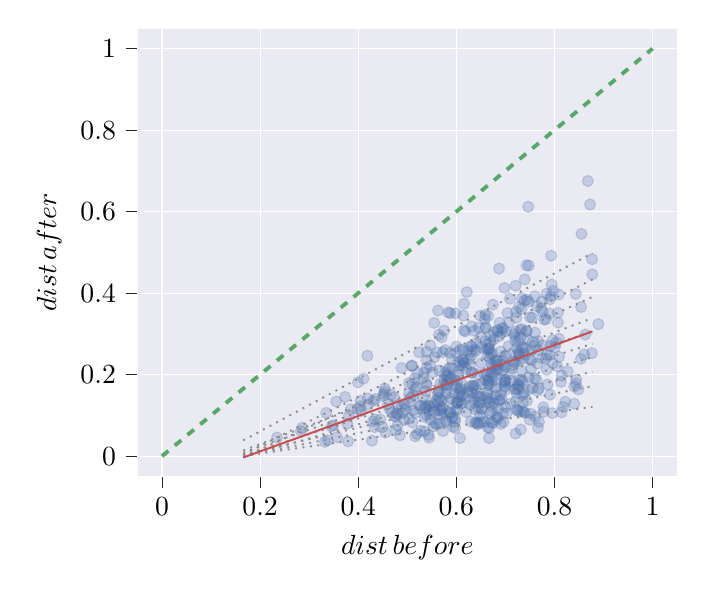
\begin{tikzpicture}

\definecolor{color0}{rgb}{0.917647058823529,0.917647058823529,0.949019607843137}
\definecolor{color1}{rgb}{0.298039215686275,0.447058823529412,0.690196078431373}
\definecolor{color2}{rgb}{0.768627450980392,0.305882352941176,0.32156862745098}
\definecolor{color3}{rgb}{0.333333333333333,0.658823529411765,0.407843137254902}

\begin{axis}[
axis background/.style={fill=color0},
axis line style={white},
tick align=outside,
tick pos=left,
x grid style={white},
xlabel={$dist\,before$},
xmajorgrids,
xmin=-0.05, xmax=1.05,
xtick style={color=white!15!black},
y grid style={white},
ylabel={$dist\,after$},
ymajorgrids,
ymin=-0.05, ymax=1.05,
ytick style={color=white!15!black}
]
\addplot [only marks, mark=*, draw=color1, fill=color1, opacity=0.25, colormap/blackwhite, clip marker paths=true]
table{%
x                      y
0.641638553704997 0.174886668758842
0.68072265977141 0.148211207188502
0.403861413335875 0.122671205324769
0.554944409420659 0.326941706872856
0.737820997493874 0.107772823859426
0.7062960824742 0.269537025881534
0.613605090036171 0.235572657133985
0.720507804088671 0.305465010137321
0.673045180122014 0.121946742365167
0.754777518115756 0.340190068248883
0.738563657705241 0.381482900565754
0.631143602898985 0.318411417994272
0.56543291719272 0.20997088827363
0.590573073831948 0.0938157482904609
0.659276236841385 0.314592263808572
0.71035756411858 0.128144027114803
0.689001418478031 0.188847309522372
0.434125366847206 0.0897980042620902
0.720576246310403 0.163464165846358
0.636343727139917 0.307508052303402
0.673355463481206 0.252351533017343
0.665144816896856 0.185116136897021
0.562595356234612 0.131380613551154
0.607703458332798 0.158830715523033
0.766617293845373 0.282535352705097
0.445218411810461 0.0898520641973889
0.665485446601547 0.184670476910175
0.84344544780781 0.398070623730711
0.768607391345775 0.0839793963368448
0.716246901686102 0.231638556813073
0.692545554990023 0.140076752826749
0.698237007593022 0.412650124527259
0.377699660608192 0.0795486638981658
0.384824050454655 0.115162069746446
0.709324389674759 0.38639547016493
0.651784573563707 0.176280923767175
0.694704807540637 0.223511795385455
0.579549798000793 0.174600858380717
0.601648516056184 0.113696638596519
0.87710104416037 0.445997576982454
0.675535894272795 0.304299040911664
0.648894869885705 0.344579918097051
0.612754107218601 0.235316460236735
0.790640280613671 0.247963210501847
0.599673047121802 0.25243588712263
0.568001170616057 0.122265681297585
0.62068275832838 0.10800664937194
0.659080578277406 0.346788942667952
0.77281821893437 0.362545661910578
0.587733901486316 0.350947277922312
0.746561136671069 0.611853521417495
0.807147080091974 0.327706425440024
0.733433879259682 0.387263218606059
0.696128563700976 0.0836788207790224
0.698232645129723 0.182940099818642
0.649397821685978 0.29145617868682
0.793151848508963 0.491943726676839
0.702438697222133 0.104876083355419
0.61276289882648 0.22181159275034
0.687230346979297 0.137309947037886
0.607353664459262 0.223064797284144
0.526291954056181 0.12465617947619
0.797293285490383 0.405592443786617
0.577307709548593 0.26042220605239
0.570359230088803 0.118600842649206
0.538355011934249 0.11955588884721
0.778004527421843 0.108760381116649
0.535920076526083 0.124550748473268
0.515898327375907 0.163348500171515
0.648202774808529 0.101402182389741
0.582012468721008 0.189746087197564
0.727932472296369 0.254305218474554
0.538604266487348 0.179387181627137
0.666642937355682 0.262202615100225
0.560832535067869 0.254435543619089
0.749953441176652 0.0890977669244417
0.597861179137887 0.113063205362634
0.813158309582119 0.182474145615176
0.490426281025817 0.105846908709144
0.621310068771735 0.402432028878962
0.410844486647808 0.190012139372703
0.674103660519354 0.0813440628453471
0.679571153310731 0.165559063138366
0.634596527173236 0.132504595360842
0.725607512494434 0.17124847032644
0.608736298480042 0.136151230995487
0.739634401905101 0.250333355414127
0.631931406747132 0.269877648816827
0.808687371994969 0.396585868963783
0.707279646568497 0.328174878965779
0.854226692929035 0.365985996042343
0.503694170953704 0.179421987556102
0.357024995790821 0.0464638479902366
0.766403129163417 0.0696727645324994
0.355062679730819 0.134056662829202
0.598825077563961 0.350383648482252
0.699692246108787 0.180244753676448
0.644302592834012 0.0800097768795183
0.695298666220843 0.312983667974678
0.722014578349429 0.248513954541033
0.752330228384114 0.235233143524287
0.665604201973596 0.27493014036963
0.68381159248957 0.0945934716299996
0.684986002601592 0.118061083249048
0.60007302029352 0.268878585905255
0.728731758883264 0.109412553965711
0.405032031369455 0.136236545638476
0.698503570432173 0.245731810325365
0.650964308126329 0.266838039137796
0.563677385611134 0.157289329517754
0.698762647505227 0.170543573428355
0.658205182953496 0.336631671262865
0.876755134609899 0.483294156014171
0.658582636298773 0.0840947893591748
0.720915806514161 0.418346864195814
0.766656399867196 0.259950022277604
0.539467619773373 0.235644203673461
0.337577538749455 0.0389997118497372
0.546932646467358 0.271787190365536
0.591314971614245 0.23719028822832
0.669195297790655 0.207136355438537
0.51711432827605 0.107271065231516
0.744003224138079 0.306033483179958
0.418854988109413 0.246460145395204
0.667433701159706 0.264134629474745
0.488312169767881 0.216436199241498
0.636631872980031 0.172597416081619
0.45154447919156 0.152703211358382
0.840573624678201 0.170688762076228
0.518308393986836 0.169387497198665
0.876256906872738 0.25261358727905
0.381247640399514 0.0991218667333215
0.651007071298814 0.228694106779819
0.594930714070937 0.175126082259453
0.681837502202752 0.215573180753832
0.803377788055167 0.278463074237312
0.614012500830434 0.261029073263014
0.521226553333452 0.202582688889404
0.544551763494123 0.112338841046817
0.722963691593342 0.265468803206525
0.759157100167474 0.190800225776561
0.683829025728159 0.309197545679839
0.607567133438078 0.2615337905612
0.826847114296143 0.208017160625298
0.473125387179016 0.144522334507698
0.782675042475022 0.336148769002005
0.700625139306661 0.306473772037651
0.651273384110874 0.116938137041044
0.466254706777357 0.151164104177502
0.79563535872191 0.105440027917599
0.449334065153157 0.071267976180194
0.688376153743293 0.327554612355639
0.862899955815406 0.298208340345302
0.503937850604218 0.131842574803343
0.739594709436519 0.433830743427411
0.681905286115335 0.095862133228949
0.751481627168348 0.104244420475917
0.640033040160046 0.151289729392638
0.474439123383469 0.0993015226403645
0.66358258363943 0.246829225275411
0.334773962242152 0.106202118825728
0.671147572992874 0.293585285587019
0.587088888976542 0.19165521913122
0.634546494080785 0.141577725434159
0.720216791417084 0.282801000163085
0.630960602580191 0.247894621613651
0.727999003614568 0.236680847459381
0.755722217341008 0.167535020203368
0.711709255269955 0.185048902907336
0.672902388579237 0.203679000699461
0.671824924694845 0.110044920425968
0.620340291465176 0.212391651178859
0.4769432822768 0.09624805835528
0.539299813999573 0.216473848775296
0.588440090305114 0.108107360081157
0.60729598411036 0.0442694040605154
0.709563633442521 0.200961686042276
0.581451208429692 0.195870006731316
0.460058166917997 0.127947723912281
0.814848484237609 0.19754558085642
0.51039742118692 0.0828295640180688
0.644196220832797 0.118770238862336
0.775964374113356 0.35422409970306
0.628868944989553 0.171532883773227
0.7653369614247 0.227111255874313
0.747330581329761 0.16320874977625
0.760429540338314 0.303296708105655
0.28312556386161 0.0616440740383739
0.676318472790707 0.286528261361551
0.689629949452343 0.149606935610196
0.77902767770118 0.334974873691737
0.800936273814595 0.26708513724728
0.579691467533687 0.0880950001879989
0.659260962842759 0.282374539762818
0.508479410163913 0.221241935796559
0.669407282301661 0.27850270792226
0.713767866624843 0.215303625459298
0.727041031746082 0.282997892109074
0.663390920406625 0.15719316067325
0.601830733553028 0.132174871142034
0.747386527109746 0.193578252095234
0.719852279861062 0.23049574554226
0.721438728066763 0.353604057422018
0.790296425630466 0.349543230615318
0.668497376430559 0.140079377290197
0.567636460707652 0.114475311090045
0.721267715871165 0.134760142685503
0.681884871241144 0.225136253976958
0.720531596752482 0.292269457490086
0.463259947247329 0.11666916153502
0.524136612122111 0.254972886470565
0.687389148740667 0.212491565137454
0.615751802591631 0.374020518334841
0.66498668741305 0.343935632517887
0.608471975002521 0.165370446153669
0.427977790253302 0.0378788054780009
0.593537820839829 0.0721513457172915
0.843685396553124 0.178400281843301
0.781862160572996 0.239124424483716
0.682217333935266 0.0898164533245915
0.66191795326694 0.199054599531538
0.643237588003249 0.146291083209572
0.783836648007419 0.398494942844314
0.610208636415166 0.14681757335737
0.768234077773575 0.166275824832275
0.653032339521699 0.0933862467585584
0.545702608303429 0.104361200427944
0.646255422449235 0.129783717847058
0.597180306784572 0.0846708262467184
0.733431547756063 0.31188597744371
0.420315726645221 0.126608640591883
0.763403348818152 0.187833421090525
0.525484504701524 0.122459704624351
0.50999441830731 0.222362198022698
0.628564968695251 0.125942742446573
0.431064298138016 0.135968291669197
0.683433173399081 0.233831888125514
0.640939385312329 0.0827548537170287
0.727347340251714 0.174388577790555
0.614317969772854 0.344706914826757
0.727707285550825 0.247393104913552
0.640802312599332 0.277347236184148
0.628717745409398 0.224571264935393
0.86793565313504 0.675203144400981
0.592714539667234 0.0951180960703397
0.580739358786582 0.166028498055222
0.822235334923815 0.133657758948577
0.488285469061047 0.12078451942255
0.796555522609103 0.228005599795465
0.544364604339344 0.045158159861886
0.726107055791168 0.163777395746288
0.807014374909472 0.352028145807569
0.740206455347533 0.106194555119733
0.560110759184686 0.0786226351046871
0.750030382883057 0.340797128489435
0.574966156242422 0.308173351328733
0.6697584066814 0.250159207021677
0.379405949901145 0.0361481031779292
0.637587141996008 0.261533084948704
0.600375148020552 0.1688144245834
0.610402520373599 0.129517634991576
0.733125890015241 0.209623048159889
0.430040772905937 0.0853420062231093
0.681298467128022 0.23535450867451
0.623845763975657 0.156180420880682
0.66640277023477 0.176489728951941
0.535272501929529 0.0960727822861149
0.735609326852923 0.132560762079124
0.735167351442082 0.183296348773239
0.572734458686764 0.255162796276433
0.675972206431502 0.129362731400231
0.724330334956628 0.176263204625864
0.735990557828617 0.238260394925131
0.493754883926366 0.127949334444629
0.667336103253995 0.132050224562194
0.419659921595979 0.141331410464967
0.643614568260151 0.201432464680796
0.480952115079872 0.10264897956603
0.62972833933512 0.0850273814777647
0.587449121310729 0.253669657230674
0.577047019388422 0.204536706630604
0.760865403767617 0.270581402670704
0.679973800917465 0.169538405127698
0.661773923467024 0.263059026638511
0.690285907546172 0.25643322518726
0.665352404015593 0.17581503969303
0.687061670897792 0.460469874417677
0.665303128294898 0.133405756985703
0.666551234904606 0.0443590181149324
0.511364550695296 0.112288294248763
0.59763792092259 0.0924616733397358
0.601329823035349 0.182654356136381
0.663149471516917 0.142284074936755
0.656678331909902 0.201912882563951
0.602541052134853 0.199486035500957
0.716142125741388 0.224846827155501
0.646829472829649 0.145829773037395
0.60182398312751 0.130280371879162
0.687768460516693 0.294614423070396
0.660225027530864 0.186600578795503
0.809471271008675 0.288029885227281
0.759992671840278 0.39191831386139
0.570158598813164 0.291645894962655
0.764086572283684 0.367483556358678
0.733090796441596 0.187529551791724
0.504117995900098 0.0926283165128716
0.840305780338122 0.128722047996378
0.519505197844307 0.0547042895047358
0.553299207219915 0.072531529346087
0.568072562235786 0.179008107473347
0.612880629934228 0.130975056219963
0.532259175878777 0.191432738262014
0.674590367818295 0.371682005103222
0.564469923184872 0.156425591942486
0.545037164883734 0.122922749306897
0.547507070053165 0.130681245324413
0.638343401069914 0.114695104924949
0.693247404355986 0.313941186459599
0.666770697179859 0.193184365250329
0.531442118454074 0.145217304067202
0.728872403692247 0.186757570232884
0.451485307900755 0.147687218761203
0.592091584291322 0.215483379356096
0.650099229536323 0.0826082100203182
0.700076322846692 0.162717812791637
0.690761883765232 0.0791177913304165
0.791126330359375 0.15099151336983
0.672797362743042 0.19051734128112
0.406181808762667 0.110940920763687
0.576021130275582 0.185612919432498
0.570066056016361 0.137889934516463
0.765703192595272 0.160559087838741
0.454557166677258 0.159461282176441
0.792589134282434 0.392403541898381
0.671883586906438 0.0831763506004329
0.579341142181717 0.153759147835019
0.559508735757534 0.136812028676611
0.699922682664247 0.219486882547011
0.534324311083996 0.204708146794913
0.678316785843946 0.233223912379702
0.674195424111798 0.220302467782162
0.625888822534808 0.237673714113475
0.785991268800028 0.175556796906385
0.73306468219812 0.361053986245059
0.79168299457156 0.270616053133438
0.848901150077598 0.163872762632543
0.692892795255488 0.303570507422353
0.585874828883757 0.216199557788642
0.889570975469532 0.323843032780717
0.596289788698352 0.187147176791817
0.643622223387014 0.0780080330888623
0.695007994925548 0.105507864605551
0.609657275118652 0.161327704812579
0.585749909635662 0.106962197465755
0.749522482677086 0.239215549190744
0.349190899214403 0.0755766705037589
0.722408553005299 0.339660871266167
0.588855163751716 0.190169845770367
0.639759464201459 0.257520006392688
0.538711499299931 0.101560314072023
0.601437964195902 0.130875063140248
0.700322599339064 0.173418013825526
0.809472771895287 0.244036981642565
0.564691378587056 0.297778627587709
0.573808991722363 0.174902089862637
0.720741046131524 0.0553625735342324
0.556377387106807 0.126184117500574
0.844424936586007 0.187933379498464
0.7447063270763 0.286650358225266
0.478795986862562 0.105284508360494
0.77564061381493 0.272535796122568
0.752199803295995 0.213747141454409
0.681168041812685 0.210886701883584
0.626000346068459 0.161074560616195
0.556209266477271 0.0812014963739457
0.505961835648657 0.143476020633513
0.737122192497355 0.265321162712034
0.481362530926205 0.126426385793212
0.615918144405854 0.229780620320323
0.695048641092843 0.210546774130985
0.604793161842668 0.208071429700068
0.555332921787635 0.109473174768429
0.700658217876529 0.188020831447909
0.669256732409862 0.104589776972627
0.572847973882361 0.0614029278358262
0.664523192140597 0.261981103639383
0.455547203885693 0.0576028436168846
0.700033429050324 0.120754399229946
0.575193293409513 0.102576953795095
0.747328353820945 0.37942519734839
0.667952246882175 0.240929944483916
0.872506138008463 0.617735929624622
0.618082209163223 0.306055337133635
0.561641660998622 0.1505083252652
0.688439946905835 0.136733395602675
0.700866983918206 0.247288629952657
0.704354102849168 0.351159721714131
0.604616508491139 0.231645656787859
0.547284699425387 0.0892536980879512
0.755675985752339 0.280042449499127
0.49397951478652 0.0885825630545125
0.722812007397028 0.153969119471216
0.727668424506357 0.365963426781398
0.579594511283019 0.084395695065214
0.631165499561902 0.205478086522407
0.345695177297644 0.073321194498158
0.736226116938119 0.151451849479096
0.551784327575209 0.205108304524657
0.855171046471625 0.545264226837479
0.730176466927857 0.309837194998493
0.534956772729605 0.0606357091190793
0.587366357215282 0.105402701214937
0.542898157130619 0.0521467946905562
0.659269057292536 0.317030146563735
0.62303734885587 0.259297212475451
0.435350895044381 0.140262412575352
0.547124510055683 0.221728965550311
0.667379226111089 0.06888402015015
0.694512222501242 0.233619179709551
0.730773233526566 0.291356376546977
0.814532515587107 0.107710026113769
0.485009602457501 0.0509905987598792
0.454187061037046 0.165757587511179
0.631195354071743 0.155498992966658
0.535058647930597 0.116892116972294
0.433583893326118 0.0709435281699772
0.633523112384598 0.169872747723697
0.537817727310961 0.159419489281222
0.645702846163803 0.315809506024488
0.50324737398292 0.152799499494937
0.468535048402587 0.106459366173369
0.597627856209884 0.0694009583253432
0.734477082998591 0.266447232395682
0.717258192816932 0.29937130944046
0.234697757830677 0.0458900250787417
0.784346009210968 0.212239152556491
0.581078391404979 0.199153169019955
0.516277733996558 0.0486113919921903
0.588601555359024 0.140960881823639
0.581165371156078 0.210422333673592
0.631480919449291 0.204745122338114
0.731368202582324 0.0652072712825389
0.663936341340342 0.0706941549036925
0.796148290686724 0.284482995778603
0.677743684797503 0.198144044071249
0.74774197107793 0.467481895793489
0.56944100847259 0.112654105674842
0.743812456182745 0.384140536129783
0.662983049008967 0.15047327629555
0.785153141679316 0.248214152284012
0.743627398325129 0.135950490014244
0.638173768778603 0.081875605127149
0.649868277997538 0.13195837090767
0.805983501707815 0.21991736923101
0.72457000786998 0.111539726085085
0.777521213497153 0.119972714813563
0.699148400613092 0.186576387334083
0.628301419893631 0.254276116743374
0.583300464416847 0.136611646373642
0.794424877302974 0.421197617006065
0.774993125557963 0.2408060830947
0.614490801311526 0.151165457544296
0.562925798344241 0.111707125605143
0.399538669202402 0.181129429041578
0.332093764527379 0.0352795315095713
0.761010252518163 0.0973647881295338
0.604961033694121 0.151786618582827
0.721348003122051 0.165321446540993
0.615700916302136 0.22894290454171
0.567667717428627 0.10435952888012
0.742139013945648 0.266039343236539
0.604357377780354 0.135961012556449
0.286151677967596 0.0698091341165861
0.596087916496712 0.1555191079695
0.774544491821953 0.379350773206806
0.510370795990827 0.176877331285928
0.742372392578552 0.30693009741434
0.527283233885947 0.0624690443789919
0.56700879700039 0.0800752734253374
0.723240545422747 0.114444099311751
0.615413545332742 0.308898664978228
0.512353389492991 0.149597909655174
0.633233690648479 0.173422047937395
0.539586605528007 0.256118899517829
0.496139446751959 0.115040339749584
0.853990146251234 0.238979570597473
0.737764066188229 0.155859553244628
0.652082559359103 0.117687024365977
0.564849086281493 0.142527008608496
0.650003524537379 0.146581316498467
0.860407073241485 0.249568166267207
0.742961940283559 0.468366716245025
0.791096068200599 0.384990985331883
0.555735235970907 0.243231135595015
0.398850883147736 0.115877892461414
0.817900307144401 0.121082535451332
0.477487564569372 0.0644432395331062
0.610546200481594 0.178940606895575
0.543330100894183 0.121934579562447
0.583534335911396 0.352452512823071
0.629245779395887 0.269627992829272
0.562833848116235 0.357207151566741
0.734029456212946 0.110515558343548
0.672034427292504 0.224859049716344
0.579779327673249 0.174656866345981
0.480042361813221 0.074950432809829
0.373047898793846 0.145353065081916
0.68471487147621 0.305981239943766
0.539934167363761 0.174164547122602
0.753423040111026 0.260117963412424
0.726898837327095 0.25348993547396
0.515547881609403 0.190777824060346
};
\addplot [line width=0.7pt, white!54.9019607843137!black, dotted]
table {%
0.165765590875884 0.000890992907985798
0.254722688422837 0.0159100103624619
0.34367978596979 0.030929027816938
0.432636883516743 0.0459480452714141
0.521593981063696 0.0609670627258903
0.610551078610649 0.0759860801803664
0.699508176157603 0.0910050976348425
0.788465273704556 0.106024115089319
0.877422371251509 0.121043132543795
};
\addplot [line width=0.7pt, white!54.9019607843137!black, dotted]
table {%
0.165765590875884 -0.000188538189394939
0.254722688422837 0.0213172326598025
0.34367978596979 0.0428230035089999
0.432636883516743 0.0643287743581973
0.521593981063696 0.0858345452073948
0.610551078610649 0.107340316056592
0.699508176157603 0.12884608690579
0.788465273704556 0.150351857754987
0.877422371251509 0.171857628604184
};
\addplot [line width=0.7pt, white!54.9019607843137!black, dotted]
table {%
0.165765590875884 0.00312813659182282
0.254722688422837 0.0286319136396125
0.34367978596979 0.0541356906874021
0.432636883516743 0.0796394677351918
0.521593981063696 0.105143244782981
0.610551078610649 0.130647021830771
0.699508176157603 0.156150798878561
0.788465273704556 0.18165457592635
0.877422371251509 0.20715835297414
};
\addplot [line width=0.7pt, white!54.9019607843137!black, dotted]
table {%
0.165765590875884 -0.00266813752104996
0.254722688422837 0.0280095010941632
0.34367978596979 0.0586871397093764
0.432636883516743 0.0893647783245896
0.521593981063696 0.120042416939803
0.610551078610649 0.150720055555016
0.699508176157603 0.181397694170229
0.788465273704556 0.212075332785442
0.877422371251509 0.242752971400656
};
\addplot [line width=0.7pt, white!54.9019607843137!black, dotted]
table {%
0.165765590875884 0.00231811378381767
0.254722688422837 0.0365100240781173
0.34367978596979 0.0707019343724169
0.432636883516743 0.104893844666717
0.521593981063696 0.139085754961016
0.610551078610649 0.173277665255316
0.699508176157603 0.207469575549615
0.788465273704556 0.241661485843915
0.877422371251509 0.275853396138215
};
\addplot [line width=0.7pt, white!54.9019607843137!black, dotted]
table {%
0.165765590875884 0.0088019454381091
0.254722688422837 0.0460887269670275
0.34367978596979 0.0833755084959458
0.432636883516743 0.120662290024864
0.521593981063696 0.157949071553783
0.610551078610649 0.195235853082701
0.699508176157603 0.232522634611619
0.788465273704556 0.269809416140538
0.877422371251509 0.307096197669456
};
\addplot [line width=0.7pt, white!54.9019607843137!black, dotted]
table {%
0.165765590875884 0.0139357036051997
0.254722688422837 0.0545611508726822
0.34367978596979 0.0951865981401646
0.432636883516743 0.135812045407647
0.521593981063696 0.176437492675129
0.610551078610649 0.217062939942612
0.699508176157603 0.257688387210094
0.788465273704556 0.298313834477577
0.877422371251509 0.338939281745059
};
\addplot [line width=0.7pt, white!54.9019607843137!black, dotted]
table {%
0.165765590875884 -0.00253049346500214
0.254722688422837 0.046631761788719
0.34367978596979 0.0957940170424402
0.432636883516743 0.144956272296161
0.521593981063696 0.194118527549883
0.610551078610649 0.243280782803604
0.699508176157603 0.292443038057325
0.788465273704556 0.341605293311046
0.877422371251509 0.390767548564767
};
\addplot [line width=0.7pt, white!54.9019607843137!black, dotted]
table {%
0.165765590875884 0.00433657810147507
0.254722688422837 0.0579591447605695
0.34367978596979 0.111581711419664
0.432636883516743 0.165204278078758
0.521593981063696 0.218826844737853
0.610551078610649 0.272449411396947
0.699508176157603 0.326071978056042
0.788465273704556 0.379694544715136
0.877422371251509 0.433317111374231
};
\addplot [line width=0.7pt, white!54.9019607843137!black, dotted]
table {%
0.165765590875884 0.0388219906523009
0.254722688422837 0.0962653190879389
0.34367978596979 0.153708647523577
0.432636883516743 0.211151975959215
0.521593981063696 0.268595304394853
0.610551078610649 0.326038632830491
0.699508176157603 0.383481961266129
0.788465273704556 0.440925289701767
0.877422371251509 0.498368618137405
};
\addplot [line width=0.7pt, color2]
table {%
0.165765590875884 -0.00324024308219949
0.254722688422837 0.0354200342755354
0.34367978596979 0.0740803116332703
0.432636883516743 0.112740588991005
0.521593981063696 0.15140086634874
0.610551078610649 0.190061143706475
0.699508176157603 0.22872142106421
0.788465273704556 0.267381698421945
0.877422371251509 0.30604197577968
};
\addplot [line width=1.4pt, color3, dashed]
table {%
0 0
1 1
};
\end{axis}

\end{tikzpicture}

	\caption{Quantile regression plot of 512 sampled cosine distances between target and attack article, before and after performing \acs{CW}-1000 attacks, using $\epsilon=0.05$.}
	\label{fig:curr-adv-quantile}
\end{figure}

\section{Comparison}

\begin{table}[H]
	\centering
	\begin{tabular}{ lccc } 
		\toprule		
		& \multicolumn{3}{c}{Attack} \\
		\cmidrule{2-4}
		Defense & FGSM & PGD-128 & CW-1000 \\
		\midrule
		Unsecured  						& 0.07  & 98.32 & 99.70 \\
		Adversarial Training			& 0.03  & 0.07  & 0.30 \\
		Curriculum Adversarial Training & 0.00  & 14.89 & 32.80 \\
		\bottomrule
	\end{tabular}
	\caption{Attack success rates for $rank_{min}=3$ calculated over 10,000 random article tuples (1,000 in the case of \acs{CW}) for all evaluated models and $\epsilon=0.05$.}
	\label{tab:defense-results}
\end{table}
Finally, we want to compare our achieved results between the two evaluated defense methods. Table~\ref{tab:defense-results} shows the robustness of our trained models against the targeted item-to-item attacks, performed in Chapter~\ref{chp:attacks}. We observed that using traditional \ac{AT}, we were able to significantly reduce the success rate for realistic perturbation budgets of $\epsilon\le0.05$. This result demonstrates that using adversarial examples for the training of a \ac{CNN} feature extractor can effectively increase the robustness of the model against adversarial attacks targeting the hidden feature space. Although \ac{CAT} also achieved to increase robustness in comparison to an undefended model, the increase is far lower than in the case of traditional \ac{AT}. We should note that all measured robustness metrics only indicate robustness against the type of attacks and $ \epsilon $-boundaries we tested in our experiments and are no proof for universal robustness against other unknown attacks.